\chapter{Theoretical introduction}
	
\section{Problem introduction}

General task is to predict a weather state $\Omega^t$, observed at a timestamp $t$, given $s$ steps from the past, which are essentially previous weather states: $(\Omega^{t-s \Delta d}, ..., \Omega^{t-\Delta d})=\Omega^{t-s\Delta d:t-\Delta t}$. Where $\Delta d$ is the step length, in our considerations arbitrarily chosen to be equal to 6 hours; for simplicity in further considerations we will use $\Omega^{t+1}$ instead of $\Omega^{t+\Delta d}$. We denote $\Omega^t$ as a tensor of a shape: (latitude span, longitude span, features), therefore our complete input data would be 4-dimensional with additional dimension for a time \footnote{For neural network based solutions it will be 5-dimensional due to the usage of batches.} \footnote{Additional dimension occur when using neighbor extension \ref{chap:neighbors}.}. Spatial span was selected so as to cover the border of the whole of Poland and some of its neighbors. More details regarding data are discussed in dataset chapter~\ref{chap:dataset}. High-level spatio-temporal prediction framework is presented at Figure~\ref{fig:in_out}. \\

\noindent Forecasting performance would be evaluating by objective function:
\[
    \mathcal{L}(\hat{X}, X)
\]


\newpage

\subsection{Naming convention}
 For further convenience, we propose a general naming convention. 
 \begin{table}[!h]
    \centering
     \begin{tabular}{|c|c|}
        \hline
        Symbol & Description \\
        \hline
        $\mathbf{f}$ & Set of features: $(f_1,..., f_n)$ \\
        $s$ & Number of past steps \\
        $h$ & Forecasting horizon \\
        $\Omega$ & Weather state for all features \\
        $X^t$ & $\Omega$ for timestamp t\\
        $x^t_{f_j}$ & $\Omega$ for timestamp t and feature $f_j$ \\
        $\mathbf{X}$ & $s$-element set of $\Omega$  \\
        $\hat{Y^t}$ & Prediction of $\Omega$ for timestamp t \\
        $\hat{y^t}_{f_j}$ & Prediction of $\Omega$ for timestamp t and feature $f_j$ \\
        $\mathbf{\hat{Y}}$ & $h$-element set of predicted $\Omega$ \\
        \hline
    \end{tabular}
    \caption{General conventions}
 \end{table}
 
 
%% \noindent We define a $\Phi$ as a set of baseline models that consist of: 
\begin{table}[!h]
    \centering
    \begin{tabular}{|c|c|}
        \hline
        Model Notation & Model Description \\
        \hline
        $\Phi^{es}$  & Exponential Smoothing \\
        $\Phi^{slr}$ & Simple Linear Regression \\
        $\Phi^{lr}$  & Linear Regression \\
        $\Phi^{gb}$ & Gradient Boosting Trees \\
        \hline
    \end{tabular}
\caption{Model conventions}
\end{table}

% \begin{figure}[!ht]
%     \centering

%     \begin{subfigure}[b]{0.48\textwidth}
%         \centering
%         \begin{tabular}{|c|c|}
%             \hline
%             Symbol & Description \\
%             \hline
%             $\mathbf{f}$ & Set of features: $(f_1,..., f_n)$ \\
%             $s$ & Number of past steps \\
%             $h$ & Forecasting horizon \\
%             $\Omega$ & Weather state for all features \\
%             $X_t$ & $\Omega$ for timestamp t\\
%             $\mathbf{X}$ & $s$-element set of $\Omega$  \\
%             $\hat{Y_t}$ & Prediction of $\Omega$ for timestamp t \\
%             $\mathbf{\hat{Y}}$ & $h$-element set of predicted $\Omega$ \\
%             $\hat{y_t}^{f_j}$ & Prediction of $\Omega$ for timestamp t and feature $f_j$ \\
%             \hline
%         \end{tabular}
%         \caption{General}
%     \end{subfigure}
%     % \hspace{0.05\textwidth}
%     \hspace*{\fill}
%     \begin{subfigure}[b]{0.48\textwidth}
%         \centering
%         \begin{tabular}{|c|c|}
%             \hline
%             Symbol & Description \\
%             \hline
%             $\Phi^{es}$  & Exponential Smoothing \\
%             $\Phi^{slr}$ & Simple Linear Regression \\
%             $\Phi^{lr}$  & Linear Regression \\
%             $\Phi^{gb}$ & Gradient Boosting Trees \\
%             \hline
%         \end{tabular}
%         \caption{Models}
%     \end{subfigure}

%     \caption{Naming conventions}
% \end{figure}
 
 
 \noindent It is crucial to emphasize the fact that the scale of values of distinct features is diverse. Therefore, we define a model $\Phi^i$ as a collection of independent sub-models, each exclusively responsible for predicting distinct feature $f_j$. This solution was proposed to avoid situations in which the statistical dispersion of one feature might influence the prediction of another feature.  
 \[
 \Phi^{i} = (\Phi^{i}_{f_1}, ..., \Phi^{i}_{f_n})
 \]
 In further considerations, we will use a term: sub-models for each of $\Phi^{i}_{f_j}$.

\subsection{General prediction framework}

\begin{figure}[!h]

\tikzset{every picture/.style={line width=0.75pt}} %set default line width to 0.75pt        

\begin{tikzpicture}[x=0.75pt,y=0.75pt,yscale=-1,xscale=1]
%uncomment if require: \path (0,389); %set diagram left start at 0, and has height of 389

%Shape: Cube [id:dp2816308175879604] 
\draw   (58.25,114.54) -- (81.78,91.01) -- (137.08,91.01) -- (137.08,145.91) -- (113.55,169.44) -- (58.25,169.44) -- cycle ; \draw   (137.08,91.01) -- (113.55,114.54) -- (58.25,114.54) ; \draw   (113.55,114.54) -- (113.55,169.44) ;
%Shape: Brace [id:dp4309828249836092] 
\draw   (76.63,89.37) .. controls (73.72,86.74) and (70.94,86.88) .. (68.31,89.8) -- (68.31,89.8) .. controls (64.55,93.97) and (61.21,94.73) .. (58.29,92.1) .. controls (61.21,94.73) and (60.79,98.13) .. (57.03,102.29)(58.72,100.42) -- (57.03,102.29) .. controls (54.4,105.21) and (54.54,107.99) .. (57.45,110.62) ;
%Shape: Brace [id:dp7756675475750493] 
\draw   (51.06,119.6) .. controls (46.39,119.75) and (44.14,122.16) .. (44.29,126.83) -- (44.53,134.35) .. controls (44.75,141.01) and (42.53,144.42) .. (37.86,144.57) .. controls (42.53,144.42) and (44.97,147.67) .. (45.19,154.34)(45.09,151.34) -- (45.43,161.86) .. controls (45.58,166.52) and (47.99,168.77) .. (52.66,168.62) ;
%Shape: Brace [id:dp612063156099937] 
\draw   (60.65,174.34) .. controls (60.72,179.01) and (63.09,181.3) .. (67.76,181.23) -- (76.73,181.09) .. controls (83.4,180.98) and (86.77,183.26) .. (86.84,187.93) .. controls (86.77,183.26) and (90.06,180.88) .. (96.73,180.78)(93.73,180.82) -- (105.71,180.64) .. controls (110.38,180.57) and (112.67,178.2) .. (112.6,173.53) ;
%Shape: Cube [id:dp42835259632452516] 
\draw   (201.31,112.9) -- (224.84,89.37) -- (280.14,89.37) -- (280.14,144.28) -- (256.61,167.81) -- (201.31,167.81) -- cycle ; \draw   (280.14,89.37) -- (256.61,112.9) -- (201.31,112.9) ; \draw   (256.61,112.9) -- (256.61,167.81) ;
%Shape: Brace [id:dp07592439753840141] 
\draw   (89.33,238.35) .. controls (89.33,243.02) and (91.66,245.35) .. (96.33,245.35) -- (149.81,245.35) .. controls (156.48,245.35) and (159.81,247.68) .. (159.81,252.35) .. controls (159.81,247.68) and (163.14,245.35) .. (169.81,245.35)(166.81,245.35) -- (223.29,245.35) .. controls (227.96,245.35) and (230.29,243.02) .. (230.29,238.35) ;
%Shape: Cube [id:dp7110500253196546] 
\draw   (376.35,113.72) -- (399.88,90.19) -- (455.18,90.19) -- (455.18,145.09) -- (431.65,168.62) -- (376.35,168.62) -- cycle ; \draw   (455.18,90.19) -- (431.65,113.72) -- (376.35,113.72) ; \draw   (431.65,113.72) -- (431.65,168.62) ;
%Shape: Brace [id:dp86120893233015] 
\draw   (392.33,90.19) .. controls (389.42,87.56) and (386.64,87.7) .. (384.01,90.62) -- (384.01,90.62) .. controls (380.25,94.78) and (376.91,95.54) .. (373.99,92.91) .. controls (376.91,95.54) and (376.49,98.94) .. (372.73,103.11)(374.42,101.24) -- (372.73,103.11) .. controls (370.1,106.02) and (370.24,108.8) .. (373.15,111.43) ;
%Shape: Brace [id:dp9673653209625941] 
\draw   (369.15,118.79) .. controls (364.49,118.94) and (362.24,121.34) .. (362.39,126.01) -- (362.63,133.53) .. controls (362.85,140.2) and (360.63,143.6) .. (355.96,143.75) .. controls (360.63,143.6) and (363.07,146.86) .. (363.28,153.52)(363.19,150.52) -- (363.53,161.04) .. controls (363.68,165.71) and (366.09,167.96) .. (370.75,167.81) ;
%Shape: Brace [id:dp9113296386668477] 
\draw   (378.74,173.53) .. controls (378.81,178.2) and (381.18,180.49) .. (385.85,180.42) -- (394.83,180.27) .. controls (401.5,180.17) and (404.87,182.45) .. (404.94,187.12) .. controls (404.87,182.45) and (408.16,180.07) .. (414.83,179.96)(411.83,180.01) -- (423.8,179.82) .. controls (428.47,179.75) and (430.76,177.38) .. (430.69,172.71) ;
%Shape: Cube [id:dp35039842919754816] 
\draw   (521.31,112.9) -- (544.84,89.37) -- (600.14,89.37) -- (600.14,144.28) -- (576.61,167.81) -- (521.31,167.81) -- cycle ; \draw   (600.14,89.37) -- (576.61,112.9) -- (521.31,112.9) ; \draw   (576.61,112.9) -- (576.61,167.81) ;
%Shape: Brace [id:dp3763157845274283] 
\draw   (407.33,239.35) .. controls (407.33,244.02) and (409.66,246.35) .. (414.33,246.35) -- (467.81,246.35) .. controls (474.48,246.35) and (477.81,248.68) .. (477.81,253.35) .. controls (477.81,248.68) and (481.14,246.35) .. (487.81,246.35)(484.81,246.35) -- (541.29,246.35) .. controls (545.96,246.35) and (548.29,244.02) .. (548.29,239.35) ;

% Text Node
\draw (33.24,96.31) node [anchor=north west][inner sep=0.75pt]  [rotate=-309.39,xslant=-0.03] [align=left] {{\scriptsize features}};
% Text Node
\draw (79.43,212.59) node [anchor=north west][inner sep=0.75pt]    {$X_{t}$};
% Text Node
\draw (167.65,116.51) node [anchor=north west][inner sep=0.75pt]   [align=left] {...};
% Text Node
\draw (21.86,173.65) node [anchor=north west][inner sep=0.75pt]  [rotate=-270.99] [align=left] {{\scriptsize latitude span}};
% Text Node
\draw (52.73,186.5) node [anchor=north west][inner sep=0.75pt]   [align=left] {{\scriptsize longitude span}};
% Text Node
\draw (209.49,210.96) node [anchor=north west][inner sep=0.75pt]    {$X_{t+s-1}$};
% Text Node
\draw (171.04,208.29) node [anchor=north west][inner sep=0.75pt]   [align=left] {...};
% Text Node
\draw (153.16,258.53) node [anchor=north west][inner sep=0.75pt]    {$\mathbf{X}$};
% Text Node
\draw (433.72,32.89) node [anchor=north west][inner sep=0.75pt]   [align=left] {{\Large Model Output}};
% Text Node
\draw (108.05,32.26) node [anchor=north west][inner sep=0.75pt]   [align=left] {{\Large Model Input}};
% Text Node
\draw (348.14,97.12) node [anchor=north west][inner sep=0.75pt]  [rotate=-309.39,xslant=-0.03] [align=left] {{\scriptsize features}};
% Text Node
\draw (339.95,172.84) node [anchor=north west][inner sep=0.75pt]  [rotate=-270.99] [align=left] {{\scriptsize latitude span}};
% Text Node
\draw (369.83,186.68) node [anchor=north west][inner sep=0.75pt]   [align=left] {{\scriptsize longitude span}};
% Text Node
\draw (487.65,116.51) node [anchor=north west][inner sep=0.75pt]   [align=left] {...};
% Text Node
\draw (396.43,207.59) node [anchor=north west][inner sep=0.75pt]    {$\hat{Y}_{t+s}$};
% Text Node
\draw (525.49,206.96) node [anchor=north west][inner sep=0.75pt]    {$\hat{Y}_{t+s+fh-1}$};
% Text Node
\draw (488.04,209.29) node [anchor=north west][inner sep=0.75pt]   [align=left] {...};
% Text Node
\draw (471.16,259.53) node [anchor=north west][inner sep=0.75pt]    {$\hat{\mathbf{Y}}$};


\end{tikzpicture}


\label{fig:in_out} \caption{Spatio-Temporal prediction framework} 

\end{figure}


\noindent Take into account the fact that this framework may differ when applying techniques such as grid neighbors~\ref{chap:neighbors} or using constants encodings~\ref{chap:feat_eng}. Details regarding those differences are explained deeply in subsequent chapters.

\newpage
\section{Explored techniques}
 \subsection{Autoregression}
 \noindent Each baseline model is designed to forecast the entire weather state for subsequent timestamp, with the forecasting horizon set at one. Therefore, when employing our models for short-term prediction tasks exceeding a few timestamps into the future, the autoregressive approach is commonsensical. \\ \\
 
 \noindent We denote model input as $\mathbf{X}$, a tensor of $s$ weather states: 
 \[
 \mathbf{X} = 
 \begin{bmatrix}
     X^{t} & ... & X^{t+s-1}
 \end{bmatrix}
 \]
 and output of a model as $\mathbf{\hat{Y}}$, which consist of $h$ forecasted states:
 \[
 \mathbf{\hat{Y}} = 
 \begin{bmatrix}
     \hat{Y}^{t+s} & ... & \hat{Y}^{t+s+h-1}
 \end{bmatrix}
 \]
 
 \noindent With assumption that $h \leq s$, autoregressive prediction is $h$-steps process such that:
 \begin{flalign*}
    &\hat{Y}^{t+s} = \Phi^{i}(X^{t:t+s-1}) \\
    &\hat{Y}^{t+s+1} = \Phi^{i}(X^{t+1:t+s-1}, \hat{Y}^{t+s}) \\
    &\vdots \\
    &\hat{Y}^{t+s+h-1} = \Phi^{i}(X^{t+h-1:t+s-1}, \hat{Y}^{t+s:t+s+h-2})
 \end{flalign*}

 \noindent Therefore, by simplifying:
 \[
    \mathbf{\hat{Y}} = \Phi^{i}(\mathbf{X})
 \]
 
 \noindent For each model except $\Phi^{slr}$, during every autoregressive step concatenation of outputs from sub-models is required, whereas $X_t$ needs to have information from every feature:
 \begin{flalign*}
    &\hat{y}^t_{f_j} = \Phi^{i}_{f_j}(\mathbf{X}^{t-1}) \\
    &\hat{Y}^{t} = 
    \begin{bmatrix}
        \hat{y}^t_{f_1} & ... & \hat{y}^t_{f_n}
    \end{bmatrix}
 \end{flalign*}
 
\subsection{Neighbors Extension}\label{chap:neighbors}

\noindent For every input tensor we have implemented an extension called additional neighbors. It expand each data points to include information about closely located grid boxes. Selection of neighbours is determined by the relative distance (radius) between the center of grid-boxes: $r$. In the Figure \ref{fig:neighbors}, grey-colored grid boxes represents the primary data point and black boxes represents its neighbors. \\

\begin{figure}[!ht]
    \centering
    \begin{tikzpicture}[scale=0.5]
        \draw[step=1, black] (0,0) grid (7,7);
        \filldraw[fill=gray, draw=white] (3,3) rectangle (4,4);
        \filldraw[fill=black, draw=white] (3,2) rectangle (4,3);
        \filldraw[fill=black, draw=white] (2,3) rectangle (3,4);
        \filldraw[fill=black, draw=white] (3,4) rectangle (4,5);
        \filldraw[fill=black, draw=white] (4,3) rectangle (5,4);
        
        \begin{scope}[shift={(9,0)}]
            \draw[step=1, black] (0,0) grid (7,7);
            \foreach \i in {1, ..., 9} {
                \pgfmathtruncatemacro\row{mod(\i-1,3)}
                \pgfmathtruncatemacro\col{int((\i-1)/3)}
                \filldraw[fill=black, draw=white] (\row+2,\col+2) rectangle (\row+3,\col+3);
            }
            \filldraw[fill=gray, draw=white] (3,3) rectangle (4,4);
            \filldraw[fill=black, draw=white] (1,3) rectangle (2,4);
            \filldraw[fill=black, draw=white] (5,3) rectangle (6,4);
            \filldraw[fill=black, draw=white] (3,1) rectangle (4,2);
            \filldraw[fill=black, draw=white] (3,5) rectangle (4,6);
        \end{scope}

        \begin{scope}[shift={(18,0)}]
            \draw[step=1, black] (0,0) grid (7,7);
            \foreach \i in {1, ..., 25} {
                \pgfmathtruncatemacro\row{mod(\i-1,5)}
                \pgfmathtruncatemacro\col{int((\i-1)/5)}
                \filldraw[fill=black, draw=white] (\row+1,\col+1) rectangle (\row+2,\col+2);
            }
            \filldraw[fill=gray, draw=white] (3,3) rectangle (4,4); 
            \filldraw[fill=black, draw=white] (0,3) rectangle (1,4);
            \filldraw[fill=black, draw=white] (6,3) rectangle (7,4);
            \filldraw[fill=black, draw=white] (3,0) rectangle (4,1);
            \filldraw[fill=black, draw=white] (3,6) rectangle (4,7);
        \end{scope}
    \end{tikzpicture}
    \caption{Neighbors logic for $r=(1,2,3)$}
    \label{fig:neighbors}
\end{figure}

\noindent Formal definition, assuming that grid boxes has resolution (1x1):
\begin{table}[!h]
    \centering
    \begin{tabular}{|c|c|}
        \hline
        Symbol & Description \\
        \hline
        $v_{i,j}$ & Grid box at latitude $i$ and longitude $j$ \\
        $V$  & Set of all grid boxes \\
        $\|v_{m,n} - v_{i,j}\|^2$  & Euclidian distance between centres of $v_{m,n}$ and $v_{i,j}$ \\
        $\mathcal{N}(v)$ & Set of neighbors for grid box $v$ \\
        \hline
    \end{tabular}
\end{table}
\[
    \forall v_{i,j} \in V: \{\forall v_{m,n \neq i,j} : \|v_{m,n} - v_{i,j}\|^2 \le r\} \in \mathcal{N}(v_{i,j})
\]

\noindent Unfortunately, the trade-off between memory footprint, computational complexity, and performance gain was not sufficient to incorporate and test bigger $r$ values.

 \newpage
 \section{Literature review}
 Amazing survey, use as much as possible; write the same conclusions; try to write intro similar to its abstract - distinguishing short-term weather prediction and medium-to-large weather prediction: \cite{app132112019}!!! \\ 
\noindent After stating the problem we want to shortly inspect current research and results in the field of MLWP. Therefore, we present a short review of quality papers related to this problem and broadly consider as a current state-of-the-art solutions.

\subsection{GraphCast}
\begin{figure}[!ht]
    \centering
    \includegraphics[scale=0.35]{figures/enc_pro_dec.png}
    \caption{Three main components of GraphCast \cite{lam2023graphcast}}
    \label{fig:enc_pro_dec}
\end{figure}

\noindent GraphCast, was the main inspiration for our work on the weather forecasting problem ~\cite{lam2023graphcast}. Published in late 2022 by Google Deepmind, was the first MLWP model to notably outperform state-of-the-art NWP methods (HRES) on multiple benchmarks. Furthermore, it is already being incorporated by ECMWF. The out-of-the-box approach to solving the problem by constructing a heterogeneous graph divided into 3 components: Encoder, Processor, and Decoder - Figure \ref{fig:enc_pro_dec}, with a component called Multi Mesh and multiple graph layers aggregating information from neighboring objects proved to be very successful. The architecture itself relies on the graph $\mathcal{G}$, which distinguishes 5 elements:
\begin{itemize}
    \item $\mathcal{V}^{G}$: The set of vertices of the grid,
    \item $\mathcal{V}^M$: The set of multi-mesh vertices,
    \item $\mathcal{E}^{G2M}$: The set of edges from the grid to the multi-mesh,
    \item $\mathcal{E}^{M}$: The set of edges inside the multi-mesh
    \item $\mathcal{E}^{M2G}$: The set of edges from the multi-mesh to the grid
\end{itemize} 

\noindent The authors of this solution use 474 input features, all included in $\mathcal{V}^{G}$:
\begin{itemize}
    \item Weather features: 2 timestamps of 5 surface variables and 6 atmospheric variables measured at 37 pressure levels
    \item Constants: 5 static features containing encoded spatial information as well as binary land-sea mask, geopotential, and others
    \item Forcing terms: consist of 5 encoded temporal features for 3 timestamps (one lead timestamp)
\end{itemize}

\noindent Other components have no weather context. All edges encode only spatial information such as edge lengths and coordinate differences, $\mathcal{V}^M$ encode only latitude and longitude values. The process of transferring weather knowledge to those components is discussed in subsequent subchapters.

\subsubsection{Message-passing} 
The whole essence of graph neural networks is the use of the message-passing algorithm. It is based on the aggregation of information from neighbors (usually neighboring nodes, but it can also be edges if they have features). The aggregation function must be permutation invariant - popular choices are average or sum. Example message-passing step using average function:
\[
    H_i^{t+1} = ReLU(H_i^t W \frac{1}{|\mathcal{N}(i)|} \sum_{j \in \mathcal{N}(i)} H_j^t U)
\]
\begin{table}[!h]
    \centering
    \begin{tabular}{|c|c|}
        \hline
        Symbol & Description \\
        \hline
        $H_i^t$& Neuron state at $t$ step of algorithm \\
        $W,U$ & Weight tensors \\
        $\mathcal{N}(i)$ & Set of neighbors for neuron $H_i$ \\
        \hline
    \end{tabular}
\end{table}

\subsubsection{Multi-mesh}\label{chap:multi-mesh}
The process of creating a multi-mesh involves iteratively dividing each face of the polyhedra into four parts to increase resolution: Figure \ref{fig:mesh-face}. At first, 12 vertices with uniform resolution are placed across the globe and connected by edges: $M_0$, then there are 5 iterations of the mentioned division, consequently obtaining $M_6$ with more than 40 thousand vertices: Figure \ref{fig:multi-mesh}. All generated polyhedra: $(M_0,..., M_6)$ are connected to form a multi-mesh with multiple edges of different lengths that will later be able to assimilate both short and long-distance weather contexts. \\

\begin{figure}[!ht]
    \centering
    \includegraphics[scale=0.35]{figures/multi_mesh.png}
    \caption{Simultaneous multi-mesh message-passing \cite{lam2023graphcast}}
    \label{fig:multi-mesh}
\end{figure}
\begin{figure}[!ht]
    \centering

\tikzset{every picture/.style={line width=0.75pt}} %set default line width to 0.75pt        
\begin{tikzpicture}[x=0.75pt,y=0.75pt,yscale=-1,xscale=1]
%uncomment if require: \path (0,300); %set diagram left start at 0, and has height of 300

%Shape: Triangle [id:dp5526310537518102] 
\draw   (184.18,86.13) -- (209,113.13) -- (159,113.13) -- cycle ;
%Straight Lines [id:da5309512728134356] 
\draw    (184,113.13) -- (171,100.13) ;
%Straight Lines [id:da318567472926536] 
\draw    (171,100.13) -- (197,100.13) ;
%Straight Lines [id:da5008865323179771] 
\draw    (184,113.13) -- (197,100.13) ;
%Shape: Triangle [id:dp3052310642312507] 
\draw   (94.68,86.63) -- (119.5,113.63) -- (69.5,113.63) -- cycle ;
%Straight Lines [id:da020905912975204166] 
\draw    (125,100.13) -- (147,100.13) ;
\draw [shift={(149,100.13)}, rotate = 180] [color={rgb, 255:red, 0; green, 0; blue, 0 }  ][line width=0.75]    (10.93,-3.29) .. controls (6.95,-1.4) and (3.31,-0.3) .. (0,0) .. controls (3.31,0.3) and (6.95,1.4) .. (10.93,3.29)   ;

\end{tikzpicture}
    \caption{Multi-mesh face division}
    \label{fig:mesh-face}
\end{figure}

\subsubsection{Generation of $\mathcal{E}^{M2G}$ and $\mathcal{E}^{G2M}$}
\noindent When consider $\mathcal{V}^{G}$ as an input data and $\mathcal{V}^M$, $\mathcal{E}^{M}$ creation process is described in \ref{chap:multi-mesh} connecting these biparite graphs requires generation of $\mathcal{E}^{M2G}$ and $\mathcal{E}^{G2M}$.\\

\noindent Multi-mesh refined space with the lowest resolution denoted as $M_6$ is constructed so that each face of it, specifically all three of the nodes that create such face, might be connected to the nearest grid node.\\

\noindent A reverse connection is generated when the distance between the grid node and mesh node is less or equal to 0.6 lengths of $M_6$ edge:
\[
    d_{v_i^G,v_j^M} \leq 0.6e^{M_6}
\]
It ensures that every grid point is connected with at least one mesh node.
\subsubsection{Encoder} 
At the very beginning, all graph components go through MLP layers to obtain the same latent space dimension for later convenience of information aggregation at the message-passing step. Then a single GNN layer is applied to pass weather information to the multi-mesh, updating the edge representations $\mathcal{E}^{G2M}$ by aggregating information from adjacent nodes, and updating the node representations $\mathcal{V}^M$ by aggregating all the already updated edges that arriving into particular mesh node. In addition, residual connections are applied to all components involved in this part of the algorithm.
 \begin{flalign*}
    &\mathcal{V}^{G} = MLP(\mathcal{V}^{G}) \\
    &\mathcal{V}^M = MLP(\mathcal{V}^M) \\
    &\mathcal{E}^{G2M} = MLP(\mathcal{E}^{G2M}) \\
    &\mathcal{E}^{M} = MLP(\mathcal{E}^{M}) \\
    &\mathcal{E}^{M2G} = MLP(\mathcal{E}^{M2G}) \\
 \end{flalign*}

\subsubsection{Processor}
The message-passing algorithm runs similarly as in Encoder, first updating the $\mathcal{E}^M$ and then $\mathcal{V}^M$. Finally, residual connections are added identically as before. This process is iteratively called 16 times. \\

\subsubsection{Decoder}
To return to the grid and the target representation of the weather state, a graph layer is applied that updates $\mathcal{E}^{M2G}$ and $\mathcal{V}^G$ sequentially, along with the residual connections. Finally, a final MLP layer is added to change the hidden dimension to match the number of target features. \\

\subsection{MetNet}
Another notable architecture is MetNet, proposed by Google Research \cite{DBLP:journals/corr/abs-2003-12140}. It primarily aims to leverage the strengths of both convolutional and recurrent neural networks for spatio-temporal data. Architecture is divided into 3 components:
\subsubsection{Spatial Downsampler}
The component that works independently on the spatial dimension. Its task is to work as an encoder to create more compact latent space by obtaining multiple convolutional and max pooling operations that aggregate and encode spatial features of data.
\subsubsection{Temporal Encoder}
As its name suggests it focuses on temporal dimension working parallel to Spatial Downsampler. It leverages Convolutional Long Short-Term Memory (ConvLSTM) layers that emphasize the influence of the last timestamps in the input tensors. 
\subsubsection{Spatial Aggregator}
The last component functioning as a robust decoder, instead of classic MLP, incorporates axial self-attentive blocks, enabling better interpretation and knowledge aggregation \cite{ho2019axial}. \\

 \noindent An engaging strategy incorporated for the precipitation forecasting problem addressed in a paper published in 2020 - is discretizing variables into small intervals and solving instead of regression, a multi-label classification task. The motivation behind such an approach is that authors assert that the categorical distribution of data stabilizes their training process. 

\subsection{FourCastNet}
The last model that we want to refer to is FourCastNet \cite{pathak2022fourcastnet}. The motivation behind leveraging it was the tremendous increase in extreme weather events worldwide in recent years and the desire to introduce a model well-suited to high-resolution data.

\begin{figure}[!ht]
    \centering
    \includegraphics[scale=0.45]{figures/fourcastnet.png}
    \caption{FourCastNet architecture}
    \label{fig:fourcastnet}
\end{figure}


\subsubsection{Adaptive Fourier Neural Operator}

What sets it apart from its predecessors is the fact that it uses the so-called Adaptive Fourier Neural Operator (AFNO), focusing on combining the Fourier Neural Operator with a self-attention mechanism.
It also uses a vision transformer backbone that leverages the tokenization of inputs by patch embedding layer - each spatial data is converted to a sequence of $P\text{x}P$ patches, then flattened and projected into high dimensional space.
Embedded patches are later passed into a transformer encoder that allows different patches to interact with each other thanks to the attention mechanism. \\

\noindent Fourier Neural Operators can model the previously mentioned modeling interaction between each token from spatial space to Fourier space. \\

\noindent Inside the spatial mixing component, tensors are passed through the Fast Fourier Transform (FFT) with frequencies multiplied by kernels and then the inverse Fast Fourier Transform (IFFT) is performed. Due to this process of token mixing happening in Fourier space, the complexity is lower. The entire process might be called a global convolution since multiplication in Fourier space is essentially the same as convolution in spatial space. \\

\noindent The word "Adaptive" in Fourier Neural Operators mainly refers to adjusting the computational complexity even further by:
\begin{itemize}
    \item splitting a kernel of dimension $D\text{x}D$ into several separate blocks,
    \item using shared weights by each input token, which significantly reduces the number of model parameters
\end{itemize}

\noindent Because spatial data in Fourier space focused mainly on low frequencies, a sparse prior was introduced, which can be used to calculate l1 loss by so-called soft thresholding. Channel Mixing is a simple Multi-layer Perceptron that mixes spatial data in the channel dimension.

\subsubsection{Architecture}
The architecture itself consists of 12 AFNO blocks and a Linear Decoder that changes the hidden dimension to match the number of predicted features.

\noindent In addition, in the research paper, they presented a division into:
\begin{itemize}
    \item pre-training: which is a simple training that predicts 1-time step into the future
    \item fine-tuning: which calculates cost functions and performs backpropagation with autoregressive prediction taken into account
\end{itemize}

\noindent Total precipitation is extremely challenging to predict having highly sparse features and very different distribution than other features. Therefore they use it as a diagnostic variable and train it on a separate model, which uses AFNO as a backbone.

\subsubsection{Additional information}
The proposed solution is also extremely efficient in terms of computational time due to the usage of different parallelization strategies such as
\begin{itemize}
    \item data parallelism: standard batch split across GPUs,
    \item feature parallelism: TODO,
    \item spatial parallelism - TODO
\end{itemize}

\noindent The architecture achieves great results especially in predicting surface winds and hurricane intensity and paths, obtaining results similar to the IFS for short-term predictions. The proposed approach to the prediction of a very difficult feature of precipitation proved to be very good because the model obtains very satisfactory results in this area as well.

\subsection{Conclusions}
All proposed solutions exhibit both similarities and distinctions. We drew inspiration from some of these approaches and incorporated them into our model extensively described in Chapter \ref{chap:model}.

\newpage
 \section{Baselines}
 TODO: write about tensors reshaping etc. Or in preprocessing methods chapter.
 \subsection{Exponential Smoothing}
 \subsection{Simple Linear Regression}\label{chap:slinear}
 This method is essentially a basic linear regression. When predicting a particular feature $f_i$, each sub-model only considers that specific feature in the input. It is a straightforward approach that assumes no correlation between different features and like any linear regression, it follows the basic assumptions of: linearity, independence, homoscedasticity, normality, absence of multicollinearity, and absence of endogeneity. Given that our task clearly deviates from meeting most of the mentioned assumptions, this method yields results that can be considered fairly average.
\begin{flalign*}
    &\forall f_i \in \mathbf{f}: \hat{y}^t_{f_i} = \Phi^{slr}_{f_i}(x^{t-1}_{f_i})\\
    &\hat{Y}^{t} = \begin{bmatrix}
        \hat{y}^t_{f_1} & ... & \hat{y}^t_{f_n}
    \end{bmatrix}
\end{flalign*}


 \subsection{Linear Regression}\label{chap:linear}
It follows the same assumptions as \ref{chap:slinear}, but with a tweak. When forecasting the $f_i$ feature, it considers the complete weather state by using all available features as input. This indicate an assumption that different weather features might influence each other. While this approach is still naive linear model, it leads to slightly improved results. \\

  \noindent For both \ref{chap:slinear} and \ref{chap:slinear}, we have examined the performance of basic linear regression, as well as regularized versions - ridge, lasso, and elastic net. The outcomes indicate that ridge regression notably outperforms other methods. Further details are provided in the chapter \ref{chap:report}.
\begin{flalign*}
    &\forall f_i \in \mathbf{f}: \hat{y}^t_{f_i} = \Phi^{lr}_{f_i}(X^{t-1})\\
    &\hat{Y}^{t} = 
    \begin{bmatrix}
        \hat{y}^t_{f_1} & ... & \hat{y}^t_{f_n}
    \end{bmatrix} \\
\end{flalign*}
\begin{table}[!h]
    \centering
    \begin{tabular}{|c|c|}
        \hline
        Method & Loss Function \\
        \hline
        Linear & $\sum(y_i - \hat{y_i})^2$ \\
        Ridge & $\sum(y_i - \hat{y_i})^2 + \lambda \sum w_j^2$ \\
        Lasso & $\sum(y_i - \hat{y_i})^2+ \lambda \sum |w_j|$ \\
        Elastic Net & $\sum(y_i - \hat{y_i})^2 +\lambda_1 \sum w_j^2 + \lambda_2 \sum |w_j|$  \\
        \hline
    \end{tabular}
\end{table}
 
 \[
    \mathbf{X} \boldsymbol\beta = \mathbf{\hat{Y}}
 \]

 \[
    \begin{bmatrix}
    x_{11} & x_{12} & \cdots & x_{1n}\\
    x_{21} & x_{22} & \cdots & x_{2n}\\
    \vdots & \vdots & \ddots & \vdots\\
    x_{n1} & x_{n2} & \cdots & x_{nn}
    \end{bmatrix}
    \begin{bmatrix}
    \beta_1\\\beta_2\\ \vdots\\b_n
    \end{bmatrix}
    =\begin{bmatrix}
    \hat{y_1}\\\hat{y_2}\\ \vdots\\\hat{y_n}
    \end{bmatrix}
\]
 \subsection{Gradient Boosting}
Due to the state-of-the-art performance in various tabular data-related challenges and their widespread popularity, we resolve to implement and analyze solutions based on gradient boosting algorithms. We chose two widely used methods, XGBoost ~\cite{Chen_2016} and LightGBM ~\cite{ke2017lightgbm}, both delivering improved results than other baseline methods. The fundamental idea behind gradient boosting lies in the iterative construction of multiple decision trees. Using the gradient boosting algorithm, these trees are generated to improve outcomes and create a more refined representation in each successive iteration. While XGBoost and LightGBM share multiple similarities, the primary distinction lies in their tree construction processes: leaf-wise for XGBoost and level-wise for LightGBM.  \\

\noindent We also explored CatBoost ~\cite{prokhorenkova2019catboost} and classical AdaBoost algorithms. However, due to significantly longer computation times and results that did not surpass other gradient boosting methods, we decided to exclude them from the further experiments and results comparison phase.

\begin{flalign*}
    &\forall f_i \in \mathbf{f}: \hat{y}^t_{f_i} = \Phi^{gb}_{f_i}(X^{t-1})\\
    &\hat{Y}^{t} = 
    \begin{bmatrix}
        \hat{y}^t_{f_1} & ... & \hat{y}^t_{f_n}
    \end{bmatrix} \\
\end{flalign*}
\newpage
\section{Neural Network Models}
\subsection{UNet}
\begin{figure}[!h]
    \centering


\tikzset{every picture/.style={line width=0.75pt}} %set default line width to 0.75pt        

\begin{tikzpicture}[x=0.75pt,y=0.75pt,yscale=-1,xscale=1]
%uncomment if require: \path (0,555); %set diagram left start at 0, and has height of 555

%Shape: Rectangle [id:dp18715874495438933] 
\draw   (23.66,16.7) -- (26.62,16.7) -- (26.62,200.75) -- (23.66,200.75) -- cycle ;
%Shape: Rectangle [id:dp21108175618544378] 
\draw   (38.43,16.7) -- (42.8,16.7) -- (42.8,200.75) -- (38.43,200.75) -- cycle ;
%Shape: Rectangle [id:dp9926647794913771] 
\draw   (54.61,241.3) -- (58.97,241.3) -- (58.97,333.33) -- (54.61,333.33) -- cycle ;
%Shape: Rectangle [id:dp04703844440598337] 
\draw   (69.88,241.3) -- (78.61,241.3) -- (78.61,333.33) -- (69.88,333.33) -- cycle ;
%Straight Lines [id:da13135618245105463] 
\draw [color={rgb, 255:red, 38; green, 21; blue, 153 }  ,draw opacity=1 ]   (57.52,208.54) -- (57.52,219) ;
\draw [shift={(57.52,221)}, rotate = 270] [color={rgb, 255:red, 38; green, 21; blue, 153 }  ,draw opacity=1 ][line width=0.75]    (6.56,-1.97) .. controls (4.17,-0.84) and (1.99,-0.18) .. (0,0) .. controls (1.99,0.18) and (4.17,0.84) .. (6.56,1.97)   ;
%Shape: Rectangle [id:dp05141207090781941] 
\draw   (93.31,376.64) -- (102.04,376.64) -- (102.04,422.65) -- (93.31,422.65) -- cycle ;
%Shape: Rectangle [id:dp7978080816334711] 
\draw   (112.47,377.79) -- (129.92,377.79) -- (129.92,423.8) -- (112.47,423.8) -- cycle ;
%Shape: Rectangle [id:dp6479639029695707] 
\draw   (139.3,379.22) -- (156.75,379.22) -- (156.75,425.23) -- (139.3,425.23) -- cycle ;
%Shape: Rectangle [id:dp3019357955255262] 
\draw   (144.3,466.7) -- (161.75,466.7) -- (161.75,489.77) -- (144.3,489.77) -- cycle ;
%Shape: Rectangle [id:dp15769795665953923] 
\draw   (172.24,466.91) -- (202.78,466.91) -- (202.78,489.97) -- (172.24,489.97) -- cycle ;
%Shape: Rectangle [id:dp6515995363621675] 
\draw   (213.46,466.95) -- (244,466.95) -- (244,490.01) -- (213.46,490.01) -- cycle ;
%Shape: Rectangle [id:dp8944502071739182] 
\draw   (213.32,524.17) -- (243.86,524.17) -- (243.86,535.7) -- (213.32,535.7) -- cycle ;
%Shape: Rectangle [id:dp8561310330751685] 
\draw   (253.78,523.74) -- (308.31,523.74) -- (308.31,535.27) -- (253.78,535.27) -- cycle ;
%Shape: Rectangle [id:dp5055350538856822] 
\draw   (318.67,524.23) -- (373.21,524.23) -- (373.21,535.76) -- (318.67,535.76) -- cycle ;
%Straight Lines [id:da3574281493968309] 
\draw    (27.11,102.41) -- (35.72,102.41) ;
\draw [shift={(37.72,102.41)}, rotate = 180] [color={rgb, 255:red, 0; green, 0; blue, 0 }  ][line width=0.75]    (6.56,-1.97) .. controls (4.17,-0.84) and (1.99,-0.18) .. (0,0) .. controls (1.99,0.18) and (4.17,0.84) .. (6.56,1.97)   ;
%Shape: Rectangle [id:dp016488727952195026] 
\draw   (54.79,16.7) -- (59.16,16.7) -- (59.16,200.75) -- (54.79,200.75) -- cycle ;
%Straight Lines [id:da15247647004345954] 
\draw    (43.47,102.41) -- (52.08,102.41) ;
\draw [shift={(54.08,102.41)}, rotate = 180] [color={rgb, 255:red, 0; green, 0; blue, 0 }  ][line width=0.75]    (6.56,-1.97) .. controls (4.17,-0.84) and (1.99,-0.18) .. (0,0) .. controls (1.99,0.18) and (4.17,0.84) .. (6.56,1.97)   ;
%Straight Lines [id:da8673701767341216] 
\draw    (59.1,284.62) -- (67.72,284.62) ;
\draw [shift={(69.72,284.62)}, rotate = 180] [color={rgb, 255:red, 0; green, 0; blue, 0 }  ][line width=0.75]    (6.56,-1.97) .. controls (4.17,-0.84) and (1.99,-0.18) .. (0,0) .. controls (1.99,0.18) and (4.17,0.84) .. (6.56,1.97)   ;
%Straight Lines [id:da8818182844686407] 
\draw    (79.46,284.21) -- (88.08,284.21) ;
\draw [shift={(90.08,284.21)}, rotate = 180] [color={rgb, 255:red, 0; green, 0; blue, 0 }  ][line width=0.75]    (6.56,-1.97) .. controls (4.17,-0.84) and (1.99,-0.18) .. (0,0) .. controls (1.99,0.18) and (4.17,0.84) .. (6.56,1.97)   ;
%Shape: Rectangle [id:dp7536745340030019] 
\draw   (90.78,241.71) -- (99.51,241.71) -- (99.51,333.74) -- (90.78,333.74) -- cycle ;
%Straight Lines [id:da2082499344791846] 
\draw    (102.25,400.77) -- (110.07,400.77) ;
\draw [shift={(112.07,400.77)}, rotate = 180] [color={rgb, 255:red, 0; green, 0; blue, 0 }  ][line width=0.75]    (6.56,-1.97) .. controls (4.17,-0.84) and (1.99,-0.18) .. (0,0) .. controls (1.99,0.18) and (4.17,0.84) .. (6.56,1.97)   ;
%Straight Lines [id:da6021949046240975] 
\draw    (129.56,401.43) -- (137.37,401.43) ;
\draw [shift={(139.37,401.43)}, rotate = 180] [color={rgb, 255:red, 0; green, 0; blue, 0 }  ][line width=0.75]    (6.56,-1.97) .. controls (4.17,-0.84) and (1.99,-0.18) .. (0,0) .. controls (1.99,0.18) and (4.17,0.84) .. (6.56,1.97)   ;
%Straight Lines [id:da08664251038435522] 
\draw [color={rgb, 255:red, 38; green, 21; blue, 153 }  ,draw opacity=1 ]   (97.33,346.58) -- (97.33,357.03) ;
\draw [shift={(97.33,359.03)}, rotate = 270] [color={rgb, 255:red, 38; green, 21; blue, 153 }  ,draw opacity=1 ][line width=0.75]    (6.56,-1.97) .. controls (4.17,-0.84) and (1.99,-0.18) .. (0,0) .. controls (1.99,0.18) and (4.17,0.84) .. (6.56,1.97)   ;
%Straight Lines [id:da14969863750099377] 
\draw [color={rgb, 255:red, 38; green, 21; blue, 153 }  ,draw opacity=1 ]   (151.32,433.08) -- (151.32,443.54) ;
\draw [shift={(151.32,445.54)}, rotate = 270] [color={rgb, 255:red, 38; green, 21; blue, 153 }  ,draw opacity=1 ][line width=0.75]    (6.56,-1.97) .. controls (4.17,-0.84) and (1.99,-0.18) .. (0,0) .. controls (1.99,0.18) and (4.17,0.84) .. (6.56,1.97)   ;
%Straight Lines [id:da6267408337269913] 
\draw    (162.06,479.09) -- (169.87,479.09) ;
\draw [shift={(171.87,479.09)}, rotate = 180] [color={rgb, 255:red, 0; green, 0; blue, 0 }  ][line width=0.75]    (6.56,-1.97) .. controls (4.17,-0.84) and (1.99,-0.18) .. (0,0) .. controls (1.99,0.18) and (4.17,0.84) .. (6.56,1.97)   ;
%Straight Lines [id:da7106217929965524] 
\draw    (203.18,479.09) -- (210.99,479.09) ;
\draw [shift={(212.99,479.09)}, rotate = 180] [color={rgb, 255:red, 0; green, 0; blue, 0 }  ][line width=0.75]    (6.56,-1.97) .. controls (4.17,-0.84) and (1.99,-0.18) .. (0,0) .. controls (1.99,0.18) and (4.17,0.84) .. (6.56,1.97)   ;
%Straight Lines [id:da7790605040632763] 
\draw [color={rgb, 255:red, 38; green, 21; blue, 153 }  ,draw opacity=1 ]   (228.02,493.7) -- (228.02,504.15) ;
\draw [shift={(228.02,506.15)}, rotate = 270] [color={rgb, 255:red, 38; green, 21; blue, 153 }  ,draw opacity=1 ][line width=0.75]    (6.56,-1.97) .. controls (4.17,-0.84) and (1.99,-0.18) .. (0,0) .. controls (1.99,0.18) and (4.17,0.84) .. (6.56,1.97)   ;
%Straight Lines [id:da5698357539585125] 
\draw    (243.27,529.93) -- (251.09,529.93) ;
\draw [shift={(253.09,529.93)}, rotate = 180] [color={rgb, 255:red, 0; green, 0; blue, 0 }  ][line width=0.75]    (6.56,-1.97) .. controls (4.17,-0.84) and (1.99,-0.18) .. (0,0) .. controls (1.99,0.18) and (4.17,0.84) .. (6.56,1.97)   ;
%Straight Lines [id:da2416473985612968] 
\draw    (308.6,529.44) -- (316.42,529.44) ;
\draw [shift={(318.42,529.44)}, rotate = 180] [color={rgb, 255:red, 0; green, 0; blue, 0 }  ][line width=0.75]    (6.56,-1.97) .. controls (4.17,-0.84) and (1.99,-0.18) .. (0,0) .. controls (1.99,0.18) and (4.17,0.84) .. (6.56,1.97)   ;
%Straight Lines [id:da809363614141596] 
\draw [color={rgb, 255:red, 12; green, 148; blue, 38 }  ,draw opacity=1 ]   (343.63,506.58) -- (343.63,495.88) ;
\draw [shift={(343.63,493.88)}, rotate = 90] [color={rgb, 255:red, 12; green, 148; blue, 38 }  ,draw opacity=1 ][line width=0.75]    (6.56,-1.97) .. controls (4.17,-0.84) and (1.99,-0.18) .. (0,0) .. controls (1.99,0.18) and (4.17,0.84) .. (6.56,1.97)   ;
%Shape: Rectangle [id:dp025026333432921044] 
\draw   (327.98,465.72) -- (358.52,465.72) -- (358.52,488.79) -- (327.98,488.79) -- cycle ;
%Shape: Rectangle [id:dp20926001651772896] 
\draw  [fill={rgb, 255:red, 51; green, 51; blue, 51 }  ,fill opacity=0.28 ] (297.44,465.72) -- (327.98,465.72) -- (327.98,488.79) -- (297.44,488.79) -- cycle ;
%Straight Lines [id:da7562560240527322] 
\draw [color={rgb, 255:red, 51; green, 51; blue, 51 }  ,draw opacity=0.28 ][fill={rgb, 255:red, 51; green, 51; blue, 51 }  ,fill opacity=0.28 ]   (244.04,477.13) -- (262.58,477.13) -- (295.48,477.13) ;
\draw [shift={(297.48,477.13)}, rotate = 180] [color={rgb, 255:red, 51; green, 51; blue, 51 }  ,draw opacity=0.28 ][line width=0.75]    (6.56,-1.97) .. controls (4.17,-0.84) and (1.99,-0.18) .. (0,0) .. controls (1.99,0.18) and (4.17,0.84) .. (6.56,1.97)   ;
%Shape: Rectangle [id:dp8023052514571293] 
\draw   (368.55,465.68) -- (399.09,465.68) -- (399.09,488.75) -- (368.55,488.75) -- cycle ;
%Shape: Rectangle [id:dp25299169957935863] 
\draw   (409.78,465.72) -- (440.32,465.72) -- (440.32,488.79) -- (409.78,488.79) -- cycle ;
%Straight Lines [id:da701424449135518] 
\draw    (358.37,477.87) -- (366.19,477.87) ;
\draw [shift={(368.19,477.87)}, rotate = 180] [color={rgb, 255:red, 0; green, 0; blue, 0 }  ][line width=0.75]    (6.56,-1.97) .. controls (4.17,-0.84) and (1.99,-0.18) .. (0,0) .. controls (1.99,0.18) and (4.17,0.84) .. (6.56,1.97)   ;
%Straight Lines [id:da6156935246607961] 
\draw    (399.49,477.87) -- (407.31,477.87) ;
\draw [shift={(409.31,477.87)}, rotate = 180] [color={rgb, 255:red, 0; green, 0; blue, 0 }  ][line width=0.75]    (6.56,-1.97) .. controls (4.17,-0.84) and (1.99,-0.18) .. (0,0) .. controls (1.99,0.18) and (4.17,0.84) .. (6.56,1.97)   ;
%Straight Lines [id:da346111466933276] 
\draw [color={rgb, 255:red, 12; green, 148; blue, 38 }  ,draw opacity=1 ]   (424.34,444) -- (424.34,433.3) ;
\draw [shift={(424.34,431.3)}, rotate = 90] [color={rgb, 255:red, 12; green, 148; blue, 38 }  ,draw opacity=1 ][line width=0.75]    (6.56,-1.97) .. controls (4.17,-0.84) and (1.99,-0.18) .. (0,0) .. controls (1.99,0.18) and (4.17,0.84) .. (6.56,1.97)   ;
%Shape: Rectangle [id:dp3443649875713195] 
\draw   (415.23,379.22) -- (432.68,379.22) -- (432.68,425.23) -- (415.23,425.23) -- cycle ;
%Shape: Rectangle [id:dp10916547800365461] 
\draw  [fill={rgb, 255:red, 51; green, 51; blue, 51 }  ,fill opacity=0.28 ] (397.78,379.22) -- (415.23,379.22) -- (415.23,425.23) -- (397.78,425.23) -- cycle ;
%Straight Lines [id:da5453720416120884] 
\draw [color={rgb, 255:red, 51; green, 51; blue, 51 }  ,draw opacity=0.28 ][fill={rgb, 255:red, 51; green, 51; blue, 51 }  ,fill opacity=0.28 ]   (155.7,401.06) -- (174.24,401.06) -- (394.76,401.06) ;
\draw [shift={(396.76,401.06)}, rotate = 180] [color={rgb, 255:red, 51; green, 51; blue, 51 }  ,draw opacity=0.28 ][line width=0.75]    (6.56,-1.97) .. controls (4.17,-0.84) and (1.99,-0.18) .. (0,0) .. controls (1.99,0.18) and (4.17,0.84) .. (6.56,1.97)   ;
%Shape: Rectangle [id:dp7039359315516164] 
\draw   (442.93,379.01) -- (460.39,379.01) -- (460.39,425.02) -- (442.93,425.02) -- cycle ;
%Shape: Rectangle [id:dp1812213827058743] 
\draw   (469.76,379.22) -- (487.21,379.22) -- (487.21,425.23) -- (469.76,425.23) -- cycle ;
%Straight Lines [id:da8986979548500146] 
\draw    (432.72,402) -- (440.53,402) ;
\draw [shift={(442.53,402)}, rotate = 180] [color={rgb, 255:red, 0; green, 0; blue, 0 }  ][line width=0.75]    (6.56,-1.97) .. controls (4.17,-0.84) and (1.99,-0.18) .. (0,0) .. controls (1.99,0.18) and (4.17,0.84) .. (6.56,1.97)   ;
%Straight Lines [id:da7559049364738527] 
\draw    (460.02,402.65) -- (467.84,402.65) ;
\draw [shift={(469.84,402.65)}, rotate = 180] [color={rgb, 255:red, 0; green, 0; blue, 0 }  ][line width=0.75]    (6.56,-1.97) .. controls (4.17,-0.84) and (1.99,-0.18) .. (0,0) .. controls (1.99,0.18) and (4.17,0.84) .. (6.56,1.97)   ;
%Straight Lines [id:da3056268493859836] 
\draw [color={rgb, 255:red, 12; green, 148; blue, 38 }  ,draw opacity=1 ]   (477.78,354.43) -- (477.78,343.73) ;
\draw [shift={(477.78,341.73)}, rotate = 90] [color={rgb, 255:red, 12; green, 148; blue, 38 }  ,draw opacity=1 ][line width=0.75]    (6.56,-1.97) .. controls (4.17,-0.84) and (1.99,-0.18) .. (0,0) .. controls (1.99,0.18) and (4.17,0.84) .. (6.56,1.97)   ;
%Shape: Rectangle [id:dp46850395773139786] 
\draw   (473.6,240.49) -- (482.33,240.49) -- (482.33,332.51) -- (473.6,332.51) -- cycle ;
%Shape: Rectangle [id:dp8888671939844691] 
\draw  [fill={rgb, 255:red, 51; green, 51; blue, 51 }  ,fill opacity=0.28 ] (464.87,240.49) -- (473.6,240.49) -- (473.6,332.51) -- (464.87,332.51) -- cycle ;
%Straight Lines [id:da5063749890219842] 
\draw [color={rgb, 255:red, 51; green, 51; blue, 51 }  ,draw opacity=0.28 ][fill={rgb, 255:red, 51; green, 51; blue, 51 }  ,fill opacity=0.28 ]   (100.07,283.27) -- (118.61,283.27) -- (462.38,283.27) ;
\draw [shift={(464.38,283.27)}, rotate = 180] [color={rgb, 255:red, 51; green, 51; blue, 51 }  ,draw opacity=0.28 ][line width=0.75]    (6.56,-1.97) .. controls (4.17,-0.84) and (1.99,-0.18) .. (0,0) .. controls (1.99,0.18) and (4.17,0.84) .. (6.56,1.97)   ;
%Shape: Rectangle [id:dp6907443953904835] 
\draw   (493.05,240.08) -- (501.78,240.08) -- (501.78,332.1) -- (493.05,332.1) -- cycle ;
%Straight Lines [id:da05860511759288356] 
\draw    (482.27,283.39) -- (490.89,283.39) ;
\draw [shift={(492.89,283.39)}, rotate = 180] [color={rgb, 255:red, 0; green, 0; blue, 0 }  ][line width=0.75]    (6.56,-1.97) .. controls (4.17,-0.84) and (1.99,-0.18) .. (0,0) .. controls (1.99,0.18) and (4.17,0.84) .. (6.56,1.97)   ;
%Straight Lines [id:da27728843868290487] 
\draw    (502.63,282.98) -- (511.24,282.98) ;
\draw [shift={(513.24,282.98)}, rotate = 180] [color={rgb, 255:red, 0; green, 0; blue, 0 }  ][line width=0.75]    (6.56,-1.97) .. controls (4.17,-0.84) and (1.99,-0.18) .. (0,0) .. controls (1.99,0.18) and (4.17,0.84) .. (6.56,1.97)   ;
%Shape: Rectangle [id:dp5538472632746805] 
\draw   (513.95,240.49) -- (522.68,240.49) -- (522.68,332.51) -- (513.95,332.51) -- cycle ;
%Straight Lines [id:da7011046510059195] 
\draw [color={rgb, 255:red, 12; green, 148; blue, 38 }  ,draw opacity=1 ]   (519.23,220.69) -- (519.23,209.99) ;
\draw [shift={(519.23,207.99)}, rotate = 90] [color={rgb, 255:red, 12; green, 148; blue, 38 }  ,draw opacity=1 ][line width=0.75]    (6.56,-1.97) .. controls (4.17,-0.84) and (1.99,-0.18) .. (0,0) .. controls (1.99,0.18) and (4.17,0.84) .. (6.56,1.97)   ;
%Shape: Rectangle [id:dp09592051395907786] 
\draw   (518.32,17.93) -- (522.68,17.93) -- (522.68,201.98) -- (518.32,201.98) -- cycle ;
%Shape: Rectangle [id:dp43041739249131417] 
\draw  [fill={rgb, 255:red, 51; green, 51; blue, 51 }  ,fill opacity=0.28 ] (513.95,17.93) -- (518.32,17.93) -- (518.32,201.98) -- (513.95,201.98) -- cycle ;
%Straight Lines [id:da27741997849623545] 
\draw [color={rgb, 255:red, 51; green, 51; blue, 51 }  ,draw opacity=0.28 ][fill={rgb, 255:red, 51; green, 51; blue, 51 }  ,fill opacity=0.28 ]   (59.72,102.9) -- (78.26,102.9) -- (510.45,102.9) ;
\draw [shift={(512.45,102.9)}, rotate = 180] [color={rgb, 255:red, 51; green, 51; blue, 51 }  ,draw opacity=0.28 ][line width=0.75]    (6.56,-1.97) .. controls (4.17,-0.84) and (1.99,-0.18) .. (0,0) .. controls (1.99,0.18) and (4.17,0.84) .. (6.56,1.97)   ;
%Shape: Rectangle [id:dp9383922675689869] 
\draw   (533.59,17.93) -- (537.95,17.93) -- (537.95,201.98) -- (533.59,201.98) -- cycle ;
%Straight Lines [id:da22056170087348537] 
\draw    (522.26,103.63) -- (530.88,103.63) ;
\draw [shift={(532.88,103.63)}, rotate = 180] [color={rgb, 255:red, 0; green, 0; blue, 0 }  ][line width=0.75]    (6.56,-1.97) .. controls (4.17,-0.84) and (1.99,-0.18) .. (0,0) .. controls (1.99,0.18) and (4.17,0.84) .. (6.56,1.97)   ;
%Shape: Rectangle [id:dp6280810789578509] 
\draw   (549.95,17.93) -- (554.31,17.93) -- (554.31,201.98) -- (549.95,201.98) -- cycle ;
%Straight Lines [id:da06947249007810463] 
\draw    (538.62,103.63) -- (547.24,103.63) ;
\draw [shift={(549.24,103.63)}, rotate = 180] [color={rgb, 255:red, 0; green, 0; blue, 0 }  ][line width=0.75]    (6.56,-1.97) .. controls (4.17,-0.84) and (1.99,-0.18) .. (0,0) .. controls (1.99,0.18) and (4.17,0.84) .. (6.56,1.97)   ;
%Straight Lines [id:da8949476041256526] 
\draw [color={rgb, 255:red, 165; green, 39; blue, 178 }  ,draw opacity=1 ]   (553.89,103.63) -- (562.51,103.63) ;
\draw [shift={(564.51,103.63)}, rotate = 180] [color={rgb, 255:red, 165; green, 39; blue, 178 }  ,draw opacity=1 ][line width=0.75]    (6.56,-1.97) .. controls (4.17,-0.84) and (1.99,-0.18) .. (0,0) .. controls (1.99,0.18) and (4.17,0.84) .. (6.56,1.97)   ;
%Shape: Rectangle [id:dp095203997230904] 
\draw   (564.61,17.93) -- (567.58,17.93) -- (567.58,201.98) -- (564.61,201.98) -- cycle ;
%Straight Lines [id:da7888678311758952] 
\draw    (527.71,445.84) -- (536.33,445.84) ;
\draw [shift={(538.33,445.84)}, rotate = 180] [color={rgb, 255:red, 0; green, 0; blue, 0 }  ][line width=0.75]    (6.56,-1.97) .. controls (4.17,-0.84) and (1.99,-0.18) .. (0,0) .. controls (1.99,0.18) and (4.17,0.84) .. (6.56,1.97)   ;
%Straight Lines [id:da3576870770253716] 
\draw [color={rgb, 255:red, 38; green, 21; blue, 153 }  ,draw opacity=1 ]   (533.04,458.85) -- (533.04,466.18) -- (533.04,469.3) ;
\draw [shift={(533.04,471.3)}, rotate = 270] [color={rgb, 255:red, 38; green, 21; blue, 153 }  ,draw opacity=1 ][line width=0.75]    (6.56,-1.97) .. controls (4.17,-0.84) and (1.99,-0.18) .. (0,0) .. controls (1.99,0.18) and (4.17,0.84) .. (6.56,1.97)   ;
%Straight Lines [id:da9851064797865465] 
\draw [color={rgb, 255:red, 12; green, 148; blue, 38 }  ,draw opacity=1 ]   (532.86,493.08) -- (532.86,487.04) -- (532.86,482.38) ;
\draw [shift={(532.86,480.38)}, rotate = 90] [color={rgb, 255:red, 12; green, 148; blue, 38 }  ,draw opacity=1 ][line width=0.75]    (6.56,-1.97) .. controls (4.17,-0.84) and (1.99,-0.18) .. (0,0) .. controls (1.99,0.18) and (4.17,0.84) .. (6.56,1.97)   ;
%Straight Lines [id:da4818076576801169] 
\draw [color={rgb, 255:red, 51; green, 51; blue, 51 }  ,draw opacity=0.28 ]   (528.26,506.58) -- (533.53,506.58) -- (536.88,506.58) ;
\draw [shift={(538.88,506.58)}, rotate = 180] [color={rgb, 255:red, 51; green, 51; blue, 51 }  ,draw opacity=0.28 ][line width=0.75]    (6.56,-1.97) .. controls (4.17,-0.84) and (1.99,-0.18) .. (0,0) .. controls (1.99,0.18) and (4.17,0.84) .. (6.56,1.97)   ;
%Straight Lines [id:da08093937108751625] 
\draw [color={rgb, 255:red, 165; green, 39; blue, 178 }  ,draw opacity=1 ]   (528.03,524.83) -- (534.85,524.83) -- (536.64,524.83) ;
\draw [shift={(538.64,524.83)}, rotate = 180] [color={rgb, 255:red, 165; green, 39; blue, 178 }  ,draw opacity=1 ][line width=0.75]    (6.56,-1.97) .. controls (4.17,-0.84) and (1.99,-0.18) .. (0,0) .. controls (1.99,0.18) and (4.17,0.84) .. (6.56,1.97)   ;

% Text Node
\draw (10.34,116.15) node [anchor=north west][inner sep=0.75pt]  [font=\tiny,rotate=-269.46]  {$lat\times lon$};
% Text Node
\draw (35.54,2.88) node [anchor=north west][inner sep=0.75pt]  [font=\tiny]  {$u$};
% Text Node
\draw (52.25,230.52) node [anchor=north west][inner sep=0.75pt]  [font=\tiny]  {$u$};
% Text Node
\draw (30.51,300.46) node [anchor=north west][inner sep=0.75pt]  [font=\tiny,rotate=-269.46]  {$\frac{lat}{2} \times \frac{lon}{2}$};
% Text Node
\draw (67.35,229.66) node [anchor=north west][inner sep=0.75pt]  [font=\tiny]  {$2u$};
% Text Node
\draw (90.78,364.96) node [anchor=north west][inner sep=0.75pt]  [font=\tiny]  {$2u$};
% Text Node
\draw (68.68,416.08) node [anchor=north west][inner sep=0.75pt]  [font=\tiny,rotate=-269.46]  {$\frac{lat}{4} \times \frac{lon}{4}$};
% Text Node
\draw (113.96,364.92) node [anchor=north west][inner sep=0.75pt]  [font=\tiny]  {$4u$};
% Text Node
\draw (140.57,364.85) node [anchor=north west][inner sep=0.75pt]  [font=\tiny]  {$4u$};
% Text Node
\draw (146.24,451.83) node [anchor=north west][inner sep=0.75pt]  [font=\tiny]  {$4u$};
% Text Node
\draw (117.76,493.18) node [anchor=north west][inner sep=0.75pt]  [font=\tiny,rotate=-269.46]  {$\frac{lat}{8} \times \frac{lon}{8}$};
% Text Node
\draw (182.23,453.18) node [anchor=north west][inner sep=0.75pt]  [font=\tiny]  {$8u$};
% Text Node
\draw (221.28,452.81) node [anchor=north west][inner sep=0.75pt]  [font=\tiny]  {$8u$};
% Text Node
\draw (221.86,512.49) node [anchor=north west][inner sep=0.75pt]  [font=\tiny]  {$8u$};
% Text Node
\draw (183.56,547.37) node [anchor=north west][inner sep=0.75pt]  [font=\tiny,rotate=-269.46]  {$\frac{lat}{16} \times \frac{lon}{16}$};
% Text Node
\draw (271.18,512.49) node [anchor=north west][inner sep=0.75pt]  [font=\tiny]  {$16u$};
% Text Node
\draw (336.51,513.47) node [anchor=north west][inner sep=0.75pt]  [font=\tiny]  {$16u$};
% Text Node
\draw (51.9,2.88) node [anchor=north west][inner sep=0.75pt]  [font=\tiny]  {$u$};
% Text Node
\draw (88.26,229.66) node [anchor=north west][inner sep=0.75pt]  [font=\tiny]  {$2u$};
% Text Node
\draw (19.18,1.03) node [anchor=north west][inner sep=0.75pt]  [font=\tiny]  {$f$};
% Text Node
\draw (321.35,451.14) node [anchor=north west][inner sep=0.75pt]  [font=\tiny]  {$16u$};
% Text Node
\draw (378.55,451.95) node [anchor=north west][inner sep=0.75pt]  [font=\tiny]  {$8u$};
% Text Node
\draw (417.59,452.81) node [anchor=north west][inner sep=0.75pt]  [font=\tiny]  {$8u$};
% Text Node
\draw (445.51,366.14) node [anchor=north west][inner sep=0.75pt]  [font=\tiny]  {$4u$};
% Text Node
\draw (471.04,366.07) node [anchor=north west][inner sep=0.75pt]  [font=\tiny]  {$4u$};
% Text Node
\draw (408,367.29) node [anchor=north west][inner sep=0.75pt]  [font=\tiny]  {$8u$};
% Text Node
\draw (490.52,228.44) node [anchor=north west][inner sep=0.75pt]  [font=\tiny]  {$2u$};
% Text Node
\draw (511.43,228.44) node [anchor=north west][inner sep=0.75pt]  [font=\tiny]  {$2u$};
% Text Node
\draw (465.15,228.72) node [anchor=north west][inner sep=0.75pt]  [font=\tiny]  {$4u$};
% Text Node
\draw (530.69,4.1) node [anchor=north west][inner sep=0.75pt]  [font=\tiny]  {$u$};
% Text Node
\draw (547.05,4.1) node [anchor=north west][inner sep=0.75pt]  [font=\tiny]  {$u$};
% Text Node
\draw (561.23,1.65) node [anchor=north west][inner sep=0.75pt]  [font=\tiny]  {$f'$};
% Text Node
\draw (596.98,446.3) node   [align=left] {\begin{minipage}[lt]{74.17pt}\setlength\topsep{0pt}
{\tiny Conv2d 3x3, ReLU}
\end{minipage}};
% Text Node
\draw (610.58,465.84) node   [align=left] {\begin{minipage}[lt]{93.08pt}\setlength\topsep{0pt}
{\tiny \textcolor[rgb]{0.15,0.08,0.6}{MaxPool 2x2, stride=2}}
\end{minipage}};
% Text Node
\draw (596.98,485.21) node   [align=left] {\begin{minipage}[lt]{74.17pt}\setlength\topsep{0pt}
{\tiny \textcolor[rgb]{0.05,0.58,0.15}{TransposeConv2d}}
\end{minipage}};
% Text Node
\draw (598.07,507.29) node   [align=left] {\begin{minipage}[lt]{74.17pt}\setlength\topsep{0pt}
{\tiny \textcolor[rgb]{0.2,0.2,0.2}{Residual connection}}
\end{minipage}};
% Text Node
\draw (597.54,524.83) node   [align=left] {\begin{minipage}[lt]{74.17pt}\setlength\topsep{0pt}
{\tiny \textcolor[rgb]{0.65,0.15,0.7}{Conv2d 1x1}}
\end{minipage}};


\end{tikzpicture}


    \caption{UNet architecture}
    \label{fig:unet}
\end{figure}

\noindent ... each convolutional layer has 'reflect' mode to preserve exact same shape  ...

\noindent This might be consider baseline too but since achieving very high scores and sharing similar characteristics with gnn it might be described here. TODO: description of architecture.
\subsection{Main Model}\label{chap:model}
Proposed model architecture and comparision with GraphCast. \\

\noindent After briefly testing multiple Graph Convolutional Cells that support edge feature vectors, we have concluded that the most promising results and sufficient computation time are obtained by TransformerConv \cite{dwivedi2021generalization} \cite{shi2021masked}.\\
Message passing in this graph transformer operator is given by formula:
\[
    \mathbf{x}^{\prime}_i = \mathbf{W}_1 \mathbf{x}_i +
    \sum_{j \in \mathcal{N}(i)} \alpha_{i,j} \left(
    \mathbf{W}_2 \mathbf{x}_{j} + \mathbf{W}_6 \mathbf{e}_{ij}
    \right),
\]

where $\alpha_{i,j}$ is denoted as attention coefficient and computed as:
\[
    \alpha_{i,j} = \textrm{softmax} \left(
    \frac{(\mathbf{W}_3\mathbf{x}_i)^{\top}
    (\mathbf{W}_4\mathbf{x}_j + \mathbf{W}_6 \mathbf{e}_{ij})}
    {\sqrt{d}} \right)
\]

\noindent TODO: list what graph cells we've tested.

\noindent Multi-layer perceptron as an embedder converting features dimension into more abstract latent space that stores better representation of weather state.

.... \\

\noindent Multi-layer perceptron as a decoder converting encoded features into its natural representation.


\begin{flalign*}
    X = MLP^{Embedder}(X) \\
    X = GNN_1(X) \\
    ...         \\
    X = GNN_N(X) \\
    \hat{Y} = MLP^{Decoder}(X) \\
 \end{flalign*}

 \begin{flalign*}
    d_{v_i,v_j} &= \sqrt{(v_{j_x} - v_{i_x})^2 + (v_{j_y} - v_{i_y})^2} \\
    e_{v_i,v_j} &= (v_{j_x} - v_{i_x}, v_{j_y} - v_{i_y}, d_{v_i,v_j})
\end{flalign*}

\begin{figure}[!ht]

\centering


\tikzset{every picture/.style={line width=0.75pt}} %set default line width to 0.75pt        

\begin{tikzpicture}[x=0.75pt,y=0.75pt,yscale=-1,xscale=1]
%uncomment if require: \path (0,300); %set diagram left start at 0, and has height of 300

%Shape: Brace [id:dp7019805664018027] 
\draw   (292.33,79) .. controls (290.14,76.39) and (287.74,76.19) .. (285.13,78.38) -- (285.13,78.38) .. controls (281.4,81.52) and (278.44,81.79) .. (276.25,79.18) .. controls (278.44,81.79) and (277.68,84.66) .. (273.95,87.79)(275.63,86.38) -- (273.95,87.79) .. controls (271.34,89.99) and (271.14,92.39) .. (273.33,95) ;
%Straight Lines [id:da24344825121139568] 
\draw    (277.63,102.92) -- (277.63,142.92) ;
%Straight Lines [id:da6110561454804792] 
\draw    (347.7,102.78) -- (347.7,142.78) ;
%Straight Lines [id:da03871795486024654] 
\draw    (277.63,102.92) -- (347.7,102.78) ;
%Straight Lines [id:da49608827752120055] 
\draw    (277.63,142.92) -- (347.7,142.78) ;
%Straight Lines [id:da27192408985546146] 
\draw    (287.69,92.96) -- (357.66,93.08) ;
%Straight Lines [id:da3480819733752343] 
\draw    (287.69,92.96) -- (287.55,102.87) ;
%Straight Lines [id:da3901687935554585] 
\draw    (297.79,83.06) -- (367.76,83.19) ;
%Straight Lines [id:da39197446094452226] 
\draw    (297.79,83.06) -- (297.66,92.98) ;
%Straight Lines [id:da01971233582821519] 
\draw    (357.52,133.35) -- (347.61,133.35) ;
%Straight Lines [id:da8552790800436195] 
\draw    (367.34,123.41) -- (357.43,123.41) ;
%Straight Lines [id:da901598531956911] 
\draw    (357.66,93.08) -- (357.52,133.35) ;
%Straight Lines [id:da7619590199519597] 
\draw    (367.48,83.15) -- (367.34,123.41) ;
%Straight Lines [id:da8643445648605664] 
\draw    (94,115) -- (112,115) ;
\draw [shift={(114,115)}, rotate = 180] [color={rgb, 255:red, 0; green, 0; blue, 0 }  ][line width=0.75]    (10.93,-3.29) .. controls (6.95,-1.4) and (3.31,-0.3) .. (0,0) .. controls (3.31,0.3) and (6.95,1.4) .. (10.93,3.29)   ;
%Straight Lines [id:da10221146771541123] 
\draw    (492,116) -- (510,116) ;
\draw [shift={(512,116)}, rotate = 180] [color={rgb, 255:red, 0; green, 0; blue, 0 }  ][line width=0.75]    (10.93,-3.29) .. controls (6.95,-1.4) and (3.31,-0.3) .. (0,0) .. controls (3.31,0.3) and (6.95,1.4) .. (10.93,3.29)   ;
%Straight Lines [id:da5913843902335524] 
\draw    (383,115) -- (401,115) ;
\draw [shift={(403,115)}, rotate = 180] [color={rgb, 255:red, 0; green, 0; blue, 0 }  ][line width=0.75]    (10.93,-3.29) .. controls (6.95,-1.4) and (3.31,-0.3) .. (0,0) .. controls (3.31,0.3) and (6.95,1.4) .. (10.93,3.29)   ;
%Rounded Rect [id:dp0019134800479860825] 
\draw   (127,103) .. controls (127,97.48) and (131.48,93) .. (137,93) -- (212,93) .. controls (217.52,93) and (222,97.48) .. (222,103) -- (222,133) .. controls (222,138.52) and (217.52,143) .. (212,143) -- (137,143) .. controls (131.48,143) and (127,138.52) .. (127,133) -- cycle ;
%Straight Lines [id:da4758105819320845] 
\draw    (230,115) -- (248,115) ;
\draw [shift={(250,115)}, rotate = 180] [color={rgb, 255:red, 0; green, 0; blue, 0 }  ][line width=0.75]    (10.93,-3.29) .. controls (6.95,-1.4) and (3.31,-0.3) .. (0,0) .. controls (3.31,0.3) and (6.95,1.4) .. (10.93,3.29)   ;

% Text Node
\draw (288,110) node [anchor=north west][inner sep=0.75pt]  [font=\tiny] [align=left] {\begin{minipage}[lt]{28.82pt}\setlength\topsep{0pt}
\begin{center}
{\tiny Transformer }\\{\tiny Conv}
\end{center}

\end{minipage}};
% Text Node
\draw (264,57.4) node [anchor=north west][inner sep=0.75pt]    {$N$};
% Text Node
\draw (412,105.4) node [anchor=north west][inner sep=0.75pt]    {$MLP^{Decoder}$};
% Text Node
\draw (75,106.4) node [anchor=north west][inner sep=0.75pt]    {$\mathbf{X}$};
% Text Node
\draw (519,104.4) node [anchor=north west][inner sep=0.75pt]    {$\mathbf{\hat{Y}}$};
% Text Node
\draw (145,108.4) node [anchor=north west][inner sep=0.75pt]    {$Encoder$};


\end{tikzpicture}


\caption{Architecture overview}
    \label{fig:architecture}
\end{figure}

\subsection{Additional techniques and feature engineering}\label{chap:feat_eng}
Present concept of spatial-mapping, edge attributes. Explain spatial and temporal feature encodings as well as usage of constants like geopotential. 

%% \subsubsection{Constant features}
\subsubsection{Spatio-Temporal embedder}
To build a better representation of the knowledge of the weather conditions, constant/exogenous features such as geopotential, and land-sea mask were also used as a model input. In addition, with the help of the so-called Spatio-Temporal embedder - $ST^{Embedder}$, we encoded spatial and temporal information, and concatenated it in the process of forward propagation with the input feature tensor, thus obtaining a better knowledge representation for individual grid-boxes. \\

\noindent The encodings for latitude and longitude (lat,lon) of each grid box / node $v_{i,j}$ are represented as:
\[
\mathbf{u}_{geo, v_{i,j}} =
\begin{bmatrix}
    \sin{(2\pi\frac{lat}{180})} &
    \cos{(2\pi\frac{lat}{180})} &
    \sin{(2\pi\frac{lon}{360})} &
    \cos{(2\pi\frac{lon}{360})}
\end{bmatrix}
\]

\noindent Encoding of time for entire model input at timestamp $t$, where $(d, h)$ represents the day of the year and the hour in a day, is given by:
\[
\mathbf{u}_{time,t} =
\begin{bmatrix}
    \sin{(2\pi\frac{d}{365})} &
    \cos{(2\pi\frac{d}{365})} &
    \sin{(2\pi\frac{h}{24})} &
    \cos{(2\pi\frac{h}{24})}
\end{bmatrix}
\]

\noindent In the subsequent analysis, we denote the product of latitude and longitude spans as $S$. It represents the flattened spatial dimension of tensors. $B$ stands for the batch size. \\ 

\noindent The concatenation of spatio-temporal features with weather features occurs right after the input tensor passes through the $MLP^{Embedder}$ and before entering graph cells. Following the dense layer, weather representation tensor has dimensions ($B$, $S$, hidden), the $\mathbf{u}_{time}$ tensor (batch, 1, 4), and the $\mathbf{u}_{geo}$ tensor ($B$, $S$, 4). To align the corresponding dimensions of $\mathbf{u}_{time}$ it goes through another dense layer with hidden size: $S$, from which it comes out having shape: ($B$, 1, $S$), after transposing the last two dimensions we will get ($B$, $S$, 1) and ability to concatenate all 3 tensors together creating one with shape: ($B$, $S$, hidden+4+1). The concatenated tensor passes through one more dense layer ultimetaly achieving the dimension ($B$, $S$, hidden') and creating a tensor aware of spatio-temporal context. Then, the forward propagatation through the graph cells of the network occurs.

\begin{table}[!ht]
    \centering
    \begin{tabular}{|l|l|}
        \hline
        \textbf{Operation} & \textbf{Output shape} \\
        \hline
        $X = MLP^{Embedder}(X)$ & $(B, S, \text{Hidden})$ \\
        $\mathbf{u}_{time} = Dense(\mathbf{u}_{time})^{\top}$ & $(B, S, 1)$ \\
        $X = (X \oplus \mathbf{u}_{time} \oplus \mathbf{u}_{geo})$ & $(B, S, \text{Hidden} + 4 + 1)$ \\
        $X = Dense(X)$ & $(B, S, \text{Hidden'})$ \\
        \hline
    \end{tabular}
    \caption{Tensor processing through $ST^{Embedder}$ forward propagation  }
    \label{tab:st_embed}
\end{table}

\subsubsection{Spatial-Mapping}
Spatial mapping was introduced to extinguish the influence of areas near the boundaries of the input space, which were detrimental to the quality of the prediction. In the original GraphCast architecture, the data spanned the enitre globe, creating a fully connected graph; where our model utilizes data from only a small part of the globe. As the result, vertices located on the space boundaries are connected only to the inner vertices, leading to lack of weather information. Hence, we decided that in the process of training, specifically in cost function computation, and model evaluation only a subspace of the model input is employed. The concept is illustrated in the figure \ref{fig:spatial_map}, actual input dimensions are maintained.

\begin{figure}[!ht]
    \centering
    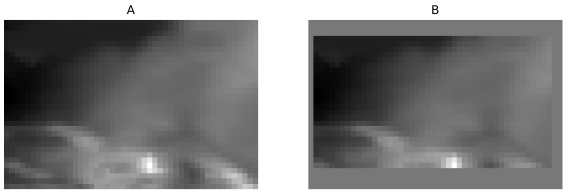
\includegraphics[scale=0.75]{figures/spatial_mapping.pdf}
    \caption{A: (32x48) Model input; B: (25x45) Mapped space}
    \label{fig:spatial_map}
\end{figure}
 